\chapter{Rivers}
\label{cha:rivers}

\section{Arquitetura}
\label{sec:rivers:architecture}

A arquitetura Rivers foi modelada com o intuito de prover uma API simples, flexível e extensível para a criação de pipelines complexos de processamento de stream de dados, tendo como fundação princípios do modelo produtor-consumidor aplicados ao modelo de concorrência da linguagem Go juntamente com o design pattern Pipeline e conceitos de programação funcional. Rivers faz uso de goroutines para o processamento concorrente e assíncrono de cada estágio do pipeline e channels para realizar a comunicação entre os mesmos. Afim de promover reuso e extensibilidade a API é definida em termos de Go interfaces disponibilizadas no pacote stream juntamente com componentes pré-definidos que podem ser combinados para criação de pipelines desde os mais simples até os mais complexos com mecanismos de fork e join por exemplo.

Rivers pipelines frequentemente são compostos por um estágio inicial conhecido como Producer \ref{sec:rivers:producers} responsável por gerar assincronamente os dados a serem processados. Opcionalmente, um pipeline pode ter um ou mais estágios intermediários conhecidos como Transformers \ref{sec:rivers:transformers} responsáveis por transformar os dados que passam por eles aplicando funções tais como filtros e flatmaps disponibilizando o resultado em um stream de leitura para que o próximo estágio possa consumi-lo de maneira assíncrona. O último estágio de um pipeline é representado por um Consumer \ref{sec:rivers:consumers} que bloqueia a execução do programa até que todos os dados sejam consumidos e o pipeline encerrado. Este último estágio ao fim da execução coleta e retorna qualquer eventual erro durante a execução para que o mesmo possa ser tratá-lo apropriadamente. Cada estágio do pipeline é conectado sequencialmente a um estágio seguinte utilizando streams de escrita e leitura conhecidos respectivamente por Writable e Readable \ref{sec:rivers:streams}. Estágios produzindo dados como producers e transformers escrevem estes valores em um stream de escrita, disponibilizando a versão de leitura deste stream à um próximo estágio para que este possa consumi-lo de maneira assíncrona.

Estágios do pipeline compartilham um mesmo contexto de execução utilizado para coordenar o fluxo de dados e sinalizar o término prematuro do pipeline devido a uma operação de short-circuit \cite{article:wikipedia:short_circuit_evaluation} ou devido a falhas ocorridas em algum ponto da execução. Este mecanismo permite com que cada estágio verifique o estado atual do pipeline antes de iniciar qualquer processamento podendo finalizar sua execução caso o pipeline tenha sido encerrado. Em situações aonde o contexto de execução é finalizado devido a erros, cada estágio do pipeline deve garantir que qualquer recurso sendo utilizado seja liberado corretamente como descritores de arquivos, channels, conexões com base de dados, etc. Um estágio pode requisitar o término do contexto de execução devido a uma falha ou pelo término prematuro como mencionado nos casos de operações de short-circuit. Este mecanismo permite que dowstreams do pipeline possam notificar upstreams com relação ao término da execução finalizando a produção de dados.

O diagrama \ref{fig:rivers:pipeline} mostra a relação entre estes componentes de um pipeline e sua representação equivalente em código Go.

\begin{figure}[H]
  \includegraphics[width=0.7\textwidth]{pipeline}
  \centering
  \caption{Rivers Pipeline.}
  \label{fig:rivers:pipeline}
\end{figure}

Pipelines podem assumir estruturas bem complexas como mencionado anteriormente. Rivers provê mecanismos para combinar múltiplos streams assim como duplicar um stream em vários outros. Estes mecanismos são conhecidos como Combiners e Dispatchers respectivamente e permitem a construção de pipelines mais complexos com vários fluxos concorrentes de processamento. Combiners são muito convenientes em situações aonde dados são produzidos por fontes de dados diferentes porém devem ser processados por uma mesma sequência de operações. O diagrama \ref{fig:rivers:combiner} representa dois pipelines sendo combinados em um único através de uma operação de merge e seu resultado sendo processado por um Transformer e em seguida consumido por um Consumer.

\begin{figure}[H]
  \includegraphics[width=0.95\textwidth]{combiner}
  \centering
  \caption{Exemplo de Uso de Combiner.}
  \label{fig:rivers:combiner}
\end{figure}

Um Dispatcher por sua vez é útil para condicionalmente classificar e separar dados de um stream os quais podem ser processados separadamente por uma sequência de estágios do pipeline. Rivers fornece algumas implementações de Dispatchers como por exemplo as operações Partition e Split. A primeira particiona o stream em dois outros baseado em um predicado que é aplicado a cada elemento do stream retornando dois novos streams. Elementos que atendem o predicados são redirecionados ao primeiro stream e o restante redirecionados ao segundo stream. A operação de Split simplesmente duplica o stream em dois outros streams idênticos permitindo que diferentes sequências de operações possam ser aplicadas a um mesmo elemento. O diagrama a seguir representa um pipeline utilizando um componente Dispatcher.

\begin{figure}[H]
  \includegraphics[width=0.85\textwidth]{dispatcher}
  \centering
  \caption{Exemplo de Uso de Dispatcher.}
  \label{fig:rivers:dispatcher}
\end{figure}

O design aplicado na implementação de Rivers visa disponibilizar uma API fluente \cite{article:martin:fluent_interfaces} similar a soluções encontradas em outras plataformas como Spark \ref{sec:apache_spark} e Java 8 Streams API \ref{sec:java8_streams}. Este estilo de API incentiva a composição de pequenos componentes com responsabilidades bem específicas afim de resolver um problema maior. O conceito de composição é bem comum no contexto de programação funcional e se encaixam de maneira muito conveniente no contexto de processamento de streams. Operações tais como filter, take, flatmap, reduce, etc permitem com que pipelines complexos sejam criados sem a necessidade de estender a API diretamente. Nos casos em que as operações nativas não sejam suficientes é possível implementar interfaces específicas para introduzir novos componentes que se comportam como por exemplo Producers, Transformers, Consumers ou qualquer outra interface disponível na API.

\section{Building Blocks}
\label{sec:rivers:building_blocks}

\subsection{Streams}
\label{sec:rivers:streams}

Streams em Rivers comportam-se como Unix pipes \ref{sec:unix_pipes}. Eles possuem uma extremidade inicial aonde dados podem ser escritos por um Producer ou Transformer por exemplo e uma extremidade final de onde dados podem ser lidos, geralmente por um Transformer ou Consumer. Streams são os conectores que permitem com que diferentes componentes do sistema sejam combinados na criação de pipelines e é por onde os dados são transmitidos de um estágio à outro podendo haver um buffer entre eles. No contexto de streams estes estágios são conhecidos como upstream e downstream respectivamente. 

Em situações em que o buffer de um stream esteja cheio, assim como no modelo Produtor-Consumidor o componente produzindo dados é bloqueado até que pelo menos um item seja consumido do buffer. De maneira análoga se o buffer estiver vazio o consumidor é bloqueado até que um novo item seja produzido e adicionado ao buffer. No contexto de streams este mecanismo bloqueante é conhecido como back pressure \ref{sec:streams:back_pressure} e é todo ele gerenciado pelo runtime da linguagem Go que também detecta situações de deadlock \ref{sec:deadlock} encerrando a execução do programa quando necessário. A figura \ref{code:stream} demonstra a criação de um stream com um buffer de capacidade 10 e um único item é escrito e em seguida lido utilizando as componentes writable e readable do stream:

\begin{figure}[H]
  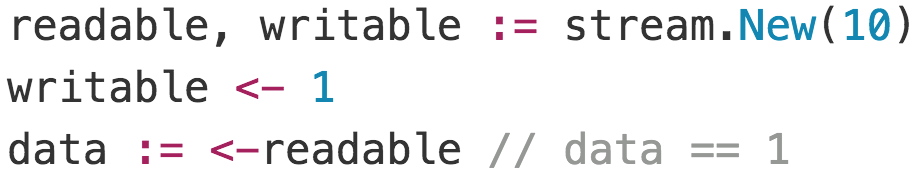
\includegraphics[width=0.55\textwidth]{stream}
  \centering
  \caption{Rivers Stream.}
  \label{code:stream}
\end{figure}

\subsection{Attachables}
\label{sec:rivers:attachable}

Componentes de um pipeline em Rivers precisam satisfazer a interface Attachable \ref{code:rivers:attachable} o que permite com que o contexto de execução atual do componente em questão seja devidamente configurado no momento em que o componente é conectado ao pipeline. É importante que os componentes de um pipeline performem sob um mesmo contexto de execução uma vez que este contexto é usado para sinalizar o término da execução devido a erros ou short-circuit operataions permitindo com que cada componente finalize sua execução apropriadamente.

\begin{figure}[H]
  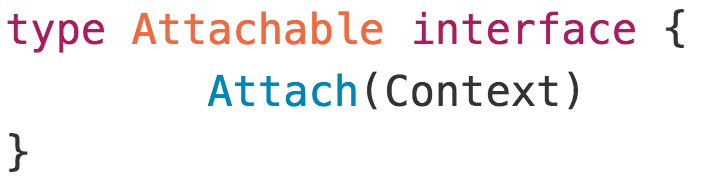
\includegraphics[width=0.4\textwidth]{attachable}
  \centering
  \caption{Attachable Interface.}
  \label{code:rivers:attachable}
\end{figure}

\subsection{Producers}
\label{sec:rivers:producers}

Producers são responsáveis pela produção de dados assincronamente disponibilizando-os em um stream de leitura que é consumido pelo estágio seguinte do pipelinem, aplicando o Pipeline Pattern \ref{subsec:pipeline_pattern}. Para utilizar um tipo como produtor de dados em um pipeline Rivers este deve implementar a interface Producer \ref{code:rivers:producer} do pacote stream, note que um Producer deve satisfazer também a interface Attachable:

\begin{figure}[H]
  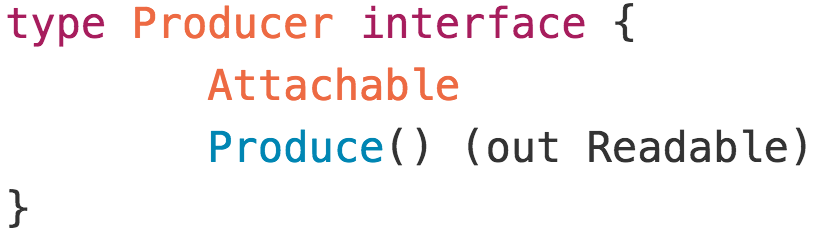
\includegraphics[width=0.45\textwidth]{producer}
  \centering
  \caption{Producer Interface.}
  \label{code:rivers:producer}
\end{figure}

Para que uma implementação de Producer possa ser utilizada em um pipeline Rivers de maneira efetiva, é necessário que o seguinte contrato seja satisfeito:

\begin{enumerate}
  \item Implementar a interface stream.Producer;
  \item Implementar o Pipeline Pattern como parte do método Produce;
  \item Como parte da goroutine produzindo dados: executar em modo defer a função Recover do contexto;
  \item Fechar a componente writable do stream uma vez que a produção de dados é encerrada;
  \item Finalizar a goroutine no caso em que o canal Done ou Failure do contexto forem fechados.
\end{enumerate}

A figura \ref{code:rivers:range_producer} mostra uma implementação de Producer que contempla o contrato anterior, produzindo números inteiros entre um intervalo pré-definido:

\begin{figure}[H]
  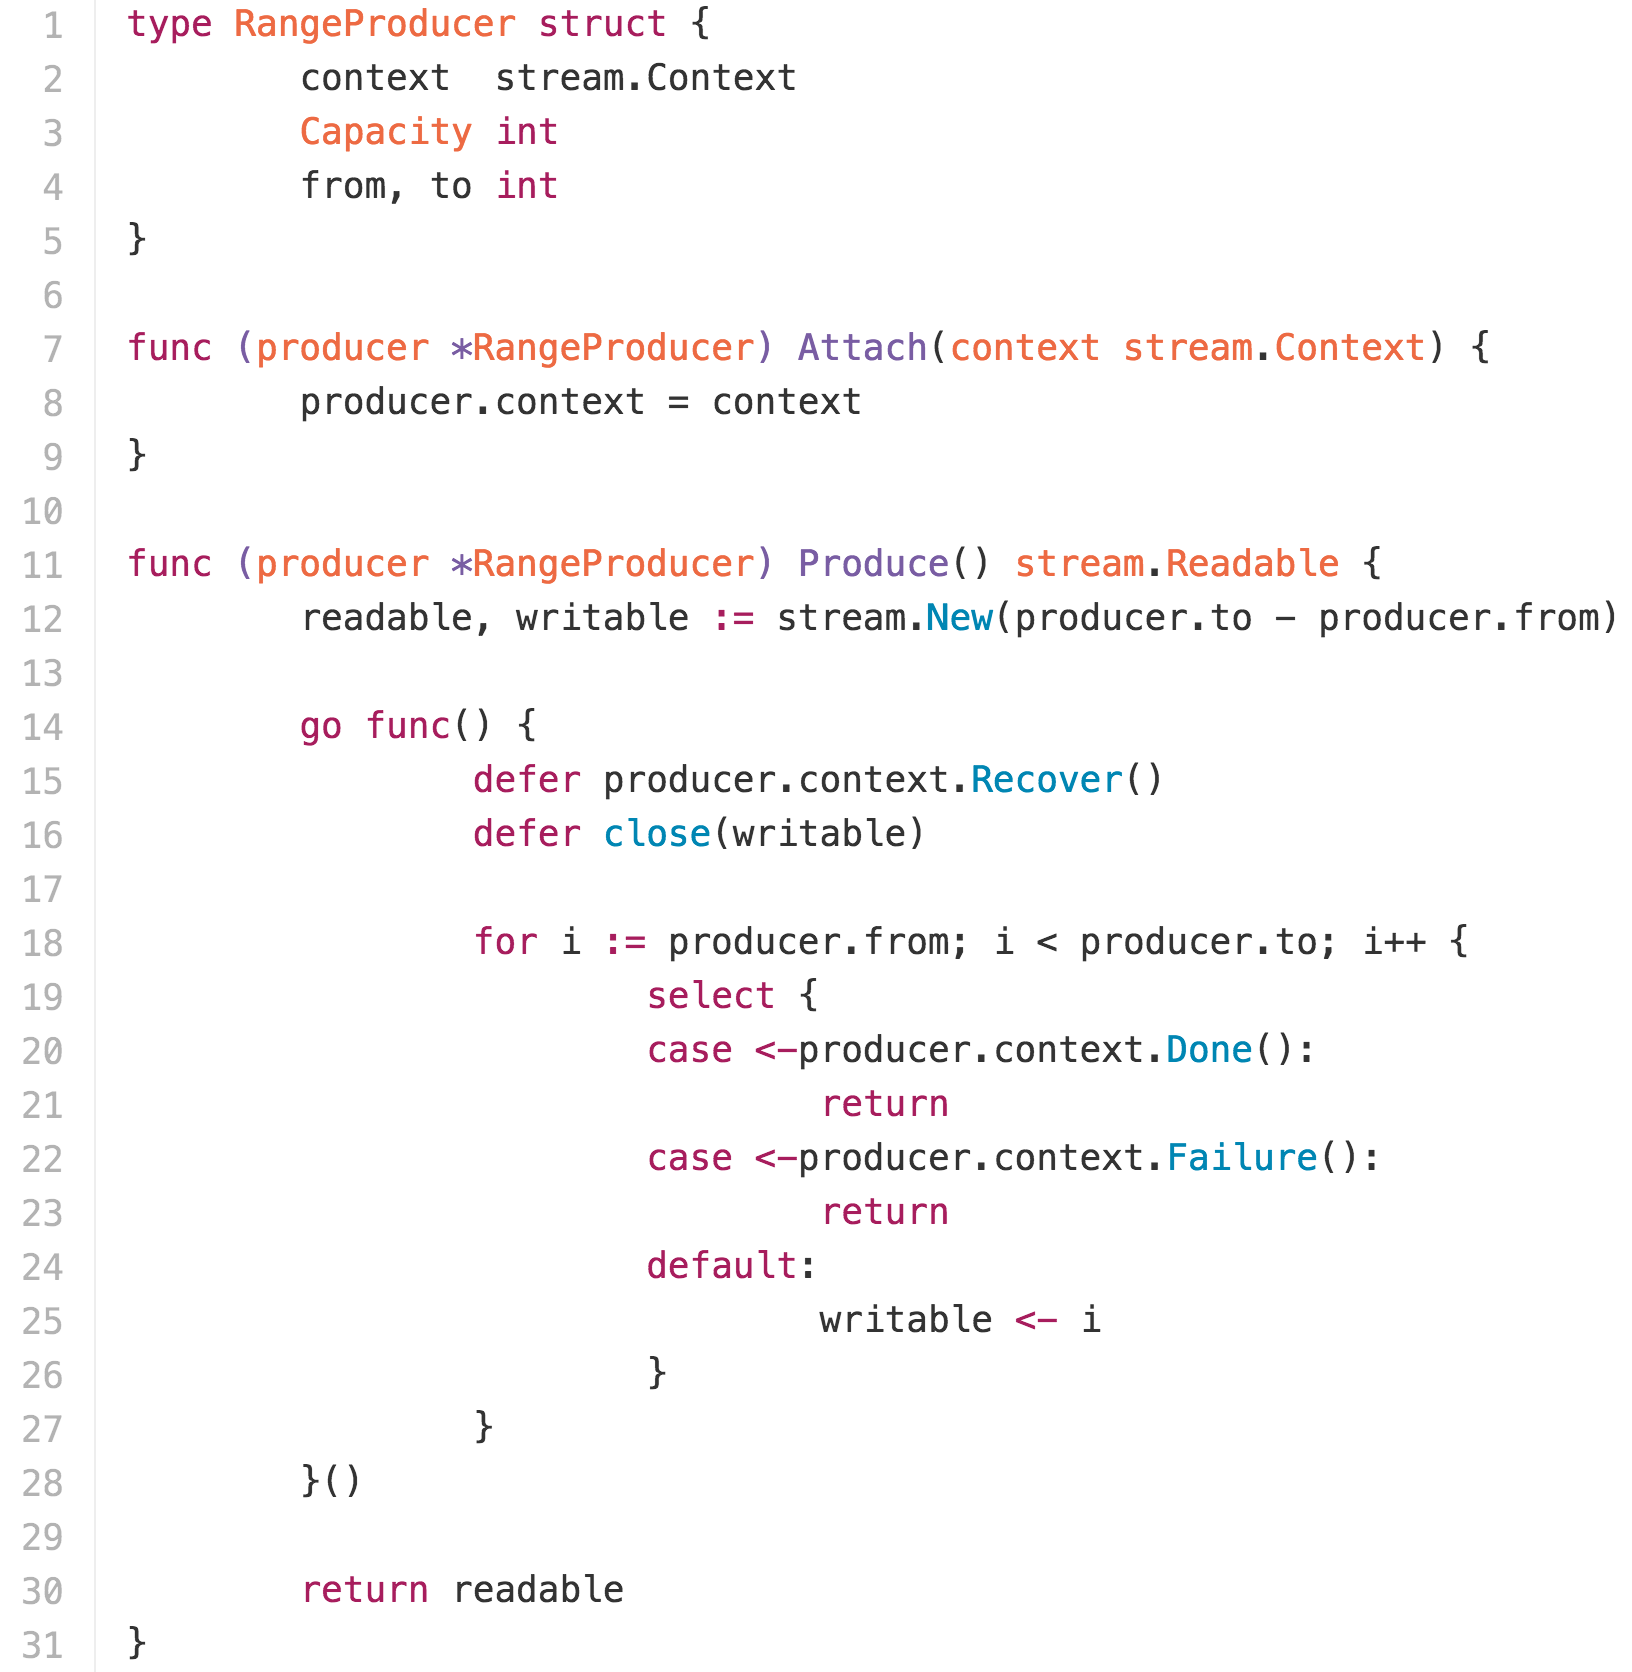
\includegraphics[width=0.95\textwidth]{range_producer}
  \centering
  \caption{Implementação de Producer que gera números inteiros entre um intervalo pré-definido.}
  \label{code:rivers:range_producer}
\end{figure}

Analisando a implementação de RangeProducer é possível verificar que o contrato anterior é implementado corretamente. Cada item do contrato é discutido a seguir:

\begin{enumerate}
\item Implementando os métodos Attach e Produce a interface stream.Producer é satisfeita;
\item O Pipeline Patter é aplicado da seguinte maneira: o método Produce cria um stream na linha 12 com capacidade igual ao quantidade de dados gerados, disparando uma goroutine na linha 14 que assincronamente escreve dados no stream através da componente writable e por fim retorna a componente readable do stream na linha 30 permitindo com que o próximo estágio do pipeline possa eventualmente consumir os dados produzidos.
\item Na linha 15 a função Recover do contexto é executada em modo defer. Isto permite com que o contexto capture e trate qualquer possível erro fatal na execução da goroutine antes que a mesma seja encerrada. Como parte da lógica de Recover, o contexto fecha o canal Failure sinalizando a falha a todos os componentes do pipeline que verificam o estado de falha ao checar o fechamento deste canal em um bloco select, linha 22.
\item Na linha 16 o fechamento da componente writable do stream é executado em modo defer. Esse passo garante que o stream será fechado mesmo em situações de erro fatal ocorridos como parte da execução da goroutine.
\item A execução da goroutine é encerrada caso algum dos canais Done linha 21 ou Failure linha 23 forem fechados. Este mecanismo de parada faz uso de uma propriedade de canais muito importante que diz que todo canal fechado está pronto para receber \ref{subsec:channels} o que faz com que o caso em particular seja selecionado no bloco select. O fechamento do canal Done indica que algum estágio do pipeline requisitou o término da execução por ter finalizado corretamente seu processamento. Esse comportamento pode ser verificado em operações de short-circuit como Find, Any que podem requisitar o término da execução por terem encontrado o resultado o final mesmo que ainda existam dados a serem produzidos. O fechamento do canal Failure por sua vez indica que algum estágio do pipeline encerrou prematuramente devido a uma falha fatal que foi capturada e tratada pela função de Recover do contexto.
\end{enumerate}

Este simples contrato permite com que diversos tipos de Producers sejam criados, simples como o exemplo anterior assim como mais complexos como por exemplo producers que geram dados de um socket, linhas de um arquivo ou até mesmo dados de uma API fornecidos através de um stream HTTP.

Afim de reduzir o boilerplate necessário na implementação de um Producer, Rivers provê o componente Observable do pacote producers que satisfaz por completo o contrato anterior reduzindo consideravelmente o número de linhas necessárias na implementação de um Producer. A implementação de RangeProducer pode ser reescrita em termos de um producers.Observable como mostrado na figura \ref{code:rivers:observable_range_producer}:

\begin{figure}[H]
  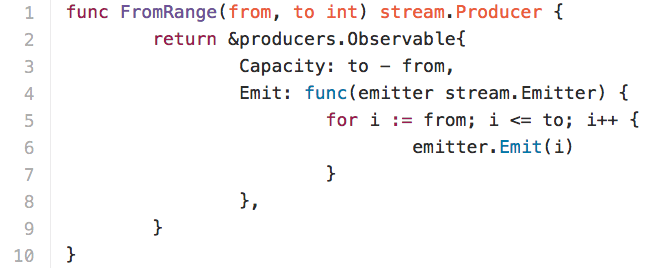
\includegraphics[width=0.8\textwidth]{observable_range_producer}
  \centering
  \caption{Implementação de RangeProducer em termos de producers.Obserbale.}
  \label{code:rivers:observable_range_producer}
\end{figure}

Todos os detalhes do contrato são encapsulados e abstraídos pelo componente Observable. A função Emit linha 4 é executada pelo próprio Observable para dar início o processo de produção dos dados e o componente emitter passado como parâmetro da função é utilizado para emitir os dados produzidos no stream, disponibilizando-os ao próximo estágio do pipeline. Rivers também disponibiliza algumas implementações pré-definidas de producers para processamento de listas, objetos, arquivos e sockets.

\subsection{Transformers}
\label{sec:rivers:transformers}

Transformers são estágios intermediários de um pipeline especializados em transformação de dados. A figura \ref{code:rivers:transformer} mostra a interface implementada por um Transformer.

\begin{figure}[H]
  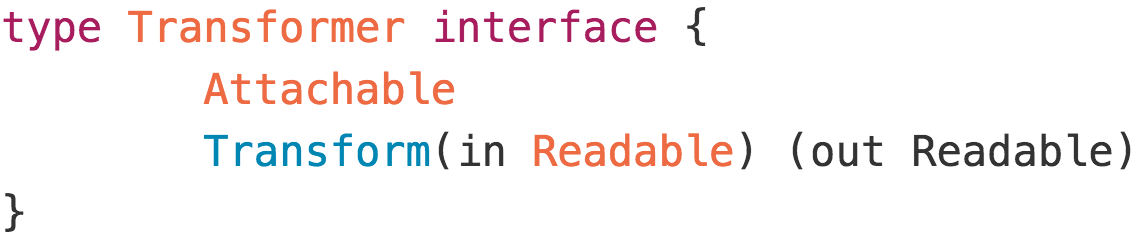
\includegraphics[width=0.6\textwidth]{transformer}
  \centering
  \caption{Transformer Interface.}
  \label{code:rivers:transformer}
\end{figure}

Uma vez conectados à um pipeline, Transformers aplicam sua função de transformação aos dados à medida que passam pelo estágio e seu resultado enviado ao próximo estágio do pipeline. Este processamento é assíncrono e implementado aplicando mais uma vez o Pipeline Pattern.

Em geral transformers são especializados e responsáveis por exercer uma função em específica no contexto de um pipeline. Vários transformers podem ser combinados para realizar lógicas de processamento mais complexas, como por exemplo uma série de filtros seguidos por transformers que acessam dados de uma API, ou banco de dados. Rivers disponibiliza várias funções de transformação pré-definidas como por exemplo Filter, Map, Each e outros.

Implementações de Transformers assim como Producers devem satisfazer um contrato que descreve os pontos necessários que uma implementação deve seguir. Estes pontos são descritos a seguir:

\begin{enumerate}
  \item Implementar a interface stream.Transformer;
  \item Implementar o Pipeline Pattern como parte do método Transform;
  \item Como parte da goroutine transformando dados: executar em modo defer a função Recover do contexto;
  \item Fechar a componente writable do stream uma vez que a transformação de dados é encerrada;
  \item Finalizar a goroutine no caso em que o canal Done ou Failure do contexto forem fechados;
  \item Finalizar a gouroutine caso não haja mais dados a serem consumidos do upstream.
\end{enumerate}

As motivações para cada item do contrato são similares as descritas com relação a implementação de um Producer. A figura \ref{code:rivers:filter_transformer} implementa um Transformer que permite com que apenas números pares sejam enviados ao estágio seguinte do pipeline, e a figura \ref{code:rivers:filter_usage}:

\begin{figure}[H]
  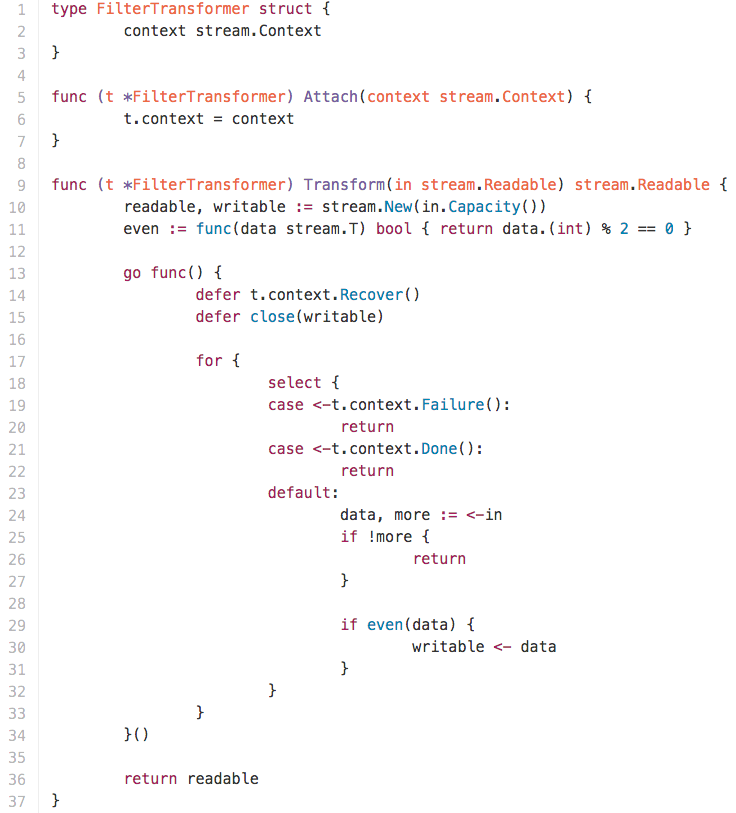
\includegraphics[width=1\textwidth]{filter_transformer}
  \centering
  \caption{Filter Transformer.}
  \label{code:rivers:filter_transformer}
\end{figure}

\begin{figure}[H]
  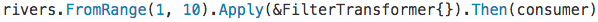
\includegraphics[width=0.85\textwidth]{filter_usage}
  \centering
  \caption{Uso do Filter Transformer em um pipeline Rivers.}
  \label{code:rivers:filter_usage}
\end{figure}

Implementações de transformers e producers são relativamente similares, com algumas restrições:

\begin{enumerate}
  \item Na linha 25 da implementação, a execução do transformer é finalizada caso não existam mais dados a serem consumidos do stream sendo transformado, neste caso o parâmetro in da função Transform;
  \item A operação de filtro é aplicada na linha 29 e dados que satisfazem a condição do filtro, neste caso números pares, são enviados ao estágio seguinte do pipeline.
\end{enumerate}

Rivers disponibiliza o tipo Observer do pacote transformers que encapsula e abstrai cada ponto do contrato mencionado anteriormente e pode ser usado como base da implementação de novos transformers, a figura seguinte reescreve o filtro anterior em termos de um Observer, e seu uso em um pipeline Rivers é mostrado na figura \ref{code:rivers:filter_observer_usage}:

\begin{figure}[H]
  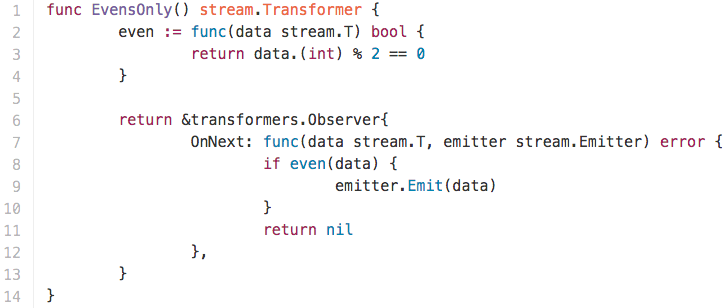
\includegraphics[width=1\textwidth]{filter_observer_transformer}
  \centering
  \caption{Filter Transformer em termos de um Observer}
  \label{code:rivers:filter_observer_transformer}
\end{figure}

\begin{figure}[H]
  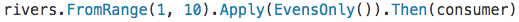
\includegraphics[width=0.75\textwidth]{filter_observer_usage}
  \centering
  \caption{Uso do EvensOnly Filter em um pipeline Rivers.}
  \label{code:rivers:filter_observer_usage}
\end{figure}

Cada dado que chega ao Transformer causa com que o método OnNext do Observer seja invocado com dois parâmetros, o dado em si e uma instância de stream.Emitter que pode ser usado para enviar dados que satisfazem o filtro ao estágio seguinte do pipeline. Caso o método OnNext retorne um erro o pipeline é encerrado e o contexto sinaliza o erro à todos os estágios fechando o channel Failure.

Filtros são operações muito úteis no processamento de streams e são essencialmente especializações de um Transformer. Por este motivo Rivers provê como parte da API mecanismos para se aplicar filtros em um stream de maneira extremamente simples, sem a necessidade de se implementar um novo Transformer. A figura \ref{code:rivers:filters_usage} mostra a aplicação de algumas implementações de filtros existentes na API.

\begin{figure}[H]
  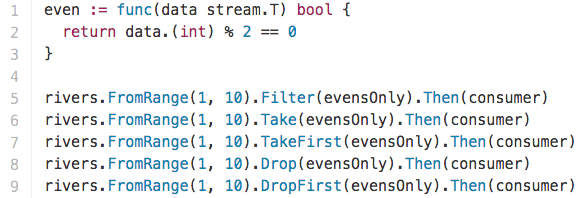
\includegraphics[width=0.85\textwidth]{filters_usage}
  \centering
  \caption{Exemplos de uso de operações de filtros.}
  \label{code:rivers:filters_usage}
\end{figure}

\subsection{Consumers}
\label{sec:rivers:consumers}

Consumers são componentes responsáveis por consumir de maneira síncrona dados de um Readable stream e representam o estágio final do pipeline, eles garantem com que o programa termine apenas ao final da execução do pipeline e reportam qualquer eventual erro de execução do mesmo. Assim como qualquer componente de um pipeline em Rivers, consumers são Attachables podendo ser conectados ao contexto de um pipeline em tempo de execução. A figura \ref{code:rivers:consumer} mostra a interface implementada por um Consumer.

\begin{figure}[H]
  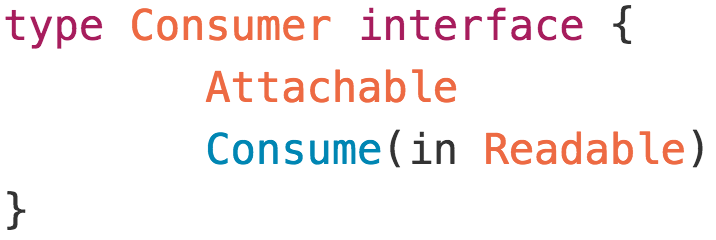
\includegraphics[width=0.35\textwidth]{consumer}
  \centering
  \caption{Consumer Interface.}
  \label{code:rivers:consumer}
\end{figure}

Consumers podem ser utilizados para realizar operações de agregamento de valores como por exemplo Count, que calcula o número total de dados que passam pelo Consumer até o final da execução do pipeline. Outra implementação útil de Consumer são os conhecidos Collectors, componentes responsáveis por coletar os dados que passam pelo consumer para serem utilizados ao final da execução do pipeline. A figura \ref{code:rivers:consumers_usage} mostra algumas aplicações de consumers em Rivers.

\begin{figure}[H]
  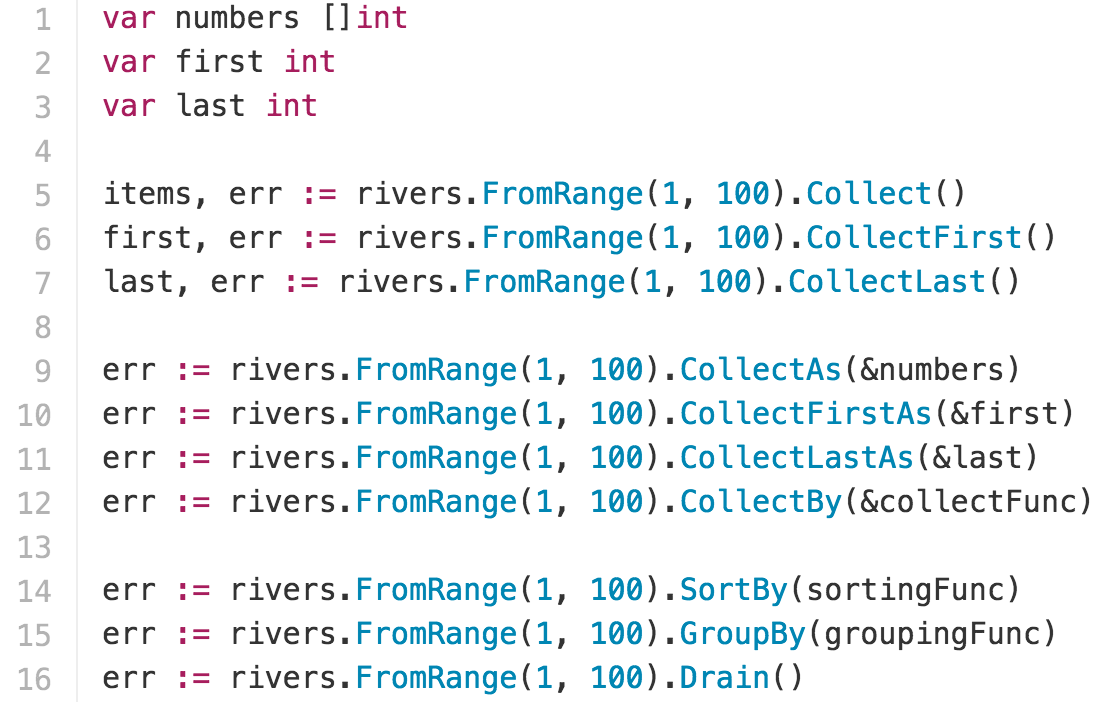
\includegraphics[width=0.75\textwidth]{consumers_usage}
  \centering
  \caption{Aplicação de consumers em Rivers.}
  \label{code:rivers:consumers_usage}
\end{figure}

Consumers ao contrário dos outros componentes do pipeline não implementam o Pipeline Pattern uma vez que estes representam estágios síncronos do pipeline e não produzem stream de dados como resultado. A figura seguir representa uma implementação simples de Consumer que realiza a operação de Count mencionada anteriormente:

\begin{figure}[H]
  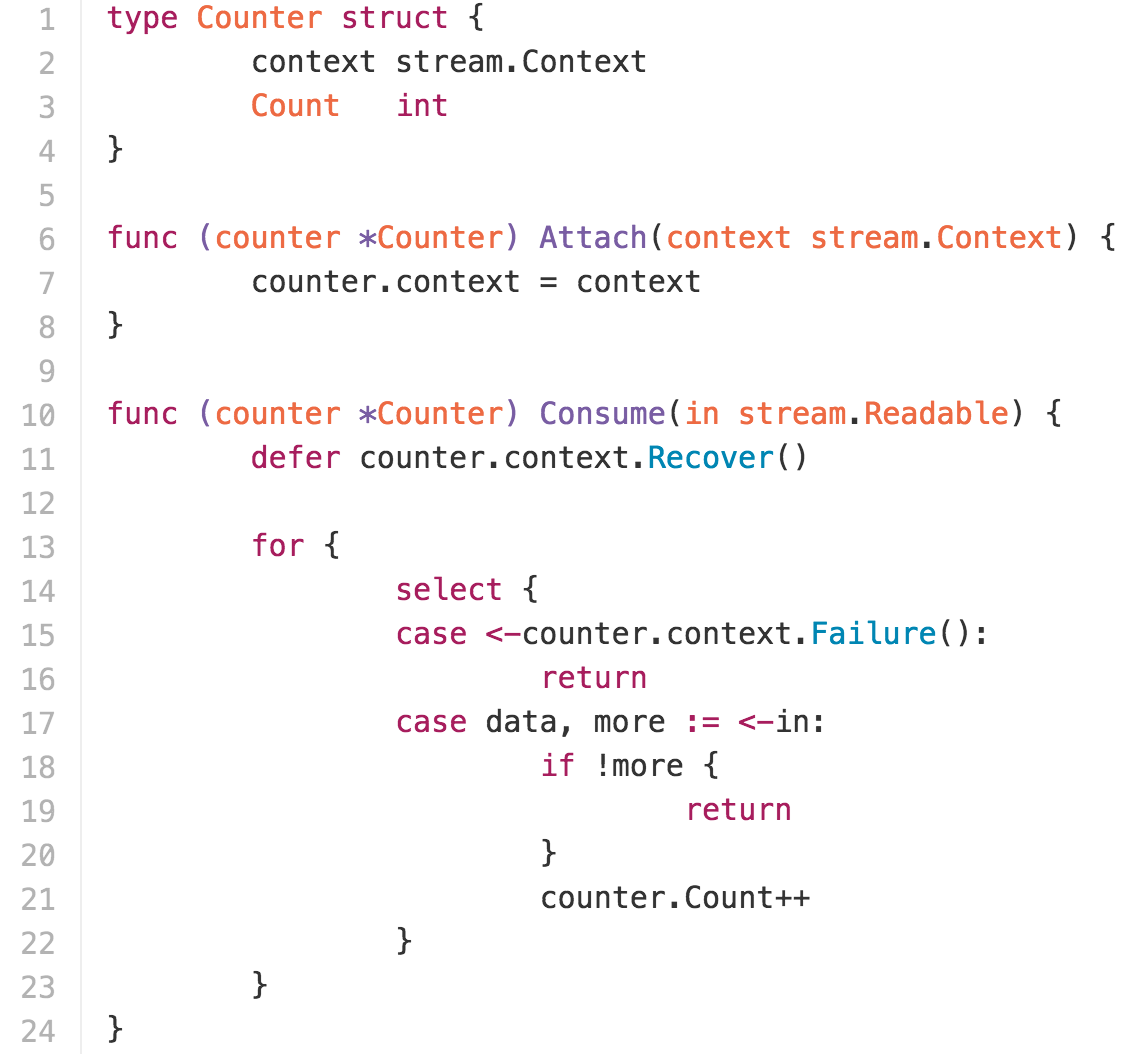
\includegraphics[width=0.75\textwidth]{consumer_count}
  \centering
  \caption{Implementação do Consumer Count.}
  \label{code:rivers:consumer_count}
\end{figure}

O contrato que uma implementação de Consumer deve seguir é relativamente simples, composto por basicamente três passos:

\begin{enumerate}
\item Executar em modo defer a função Recover do contexto como parte da implementação do método Consume;
\item Finalizar a execução caso o canal Failure do contexto foi fechado;
\item Consumir dados do Readable stream até que o stream seja encerrado.
\end{enumerate}

Apesar de simples este contrato acaba por se repetir em diversas implementações de consumers, por isso Rivers disponibiliza o tipo Sink do pacote consumers que pode ser utilizado como base na implementação de novos consumers. A implementação do Consumer Count pode ser reescrita em termos de um tipo Sink como mostrado a seguir:

\begin{figure}[H]
  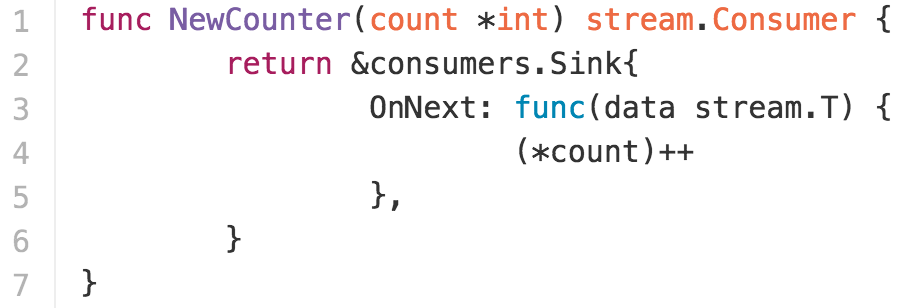
\includegraphics[width=0.6\textwidth]{consumer_count_sink}
  \centering
  \caption{Implementação do Consumer utilizando o tipo Sink como base.}
  \label{code:rivers:consumer_count_sink}
\end{figure}

\subsection{Combiners}
\label{sec:rivers:combiners}

Combiners são mecanismos utilizados para combinar assincronamente diferentes streams de dados em um único stream que pode então ser processado por estágios seguintes do pipeline. Um caso de uso seria combinar diferentes fontes de dados em um único stream, como por exemplo o resultado de uma requisição à uma API restful e uma query à um banco de dados. Os dados produzidos por cada uma dessas fontes de dados após serem combinados em um único Readable stream, podem ser processados pela mesma sequência de estágios. A figura a seguir representa a interface implementada por um Cobiner em Rivers:

\begin{figure}[H]
  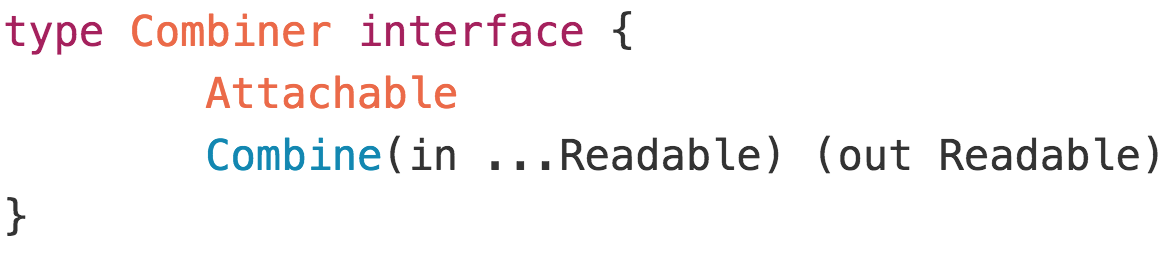
\includegraphics[width=0.6\textwidth]{combiner_interface}
  \centering
  \caption{Combiner Interface.}
  \label{code:rivers:combiner}
\end{figure}

Rivers API além de permitir com que qualquer tipo que satisfaça a interface acima possa ser utilizado como um Combiner em um pipeline, algumas implementações úteis de combiners são nativas da API e prontas para serem utilizadas como por exemplo Merge que combina dados de fontes diferentes em uma política FIFO aonde os primeiros dados que chegam de qualquer uma das fontes são imediatamente enviados para o stream final. Outra política de junção de streams é a de Zip que coleta um item de cada fonte alternadamente até que todos os dados sejam combinados, dentre outras implementações.

\begin{figure}[H]
  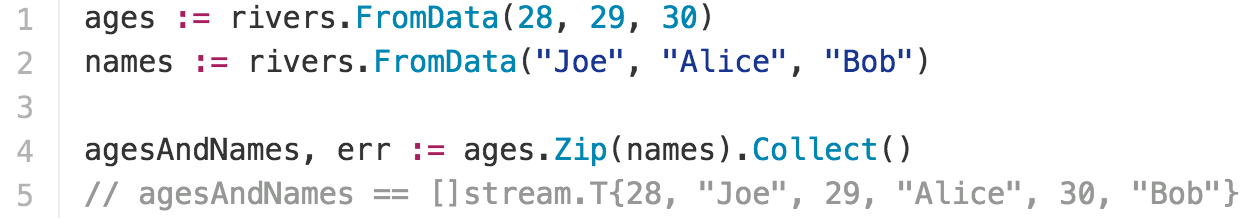
\includegraphics[width=0.9\textwidth]{zip_combiner}
  \centering
  \caption{Zip Combiner Interface.}
  \label{code:rivers:zip_combiner}
\end{figure}

\subsection{Dispatchers}
\label{sec:rivers:dispatchers}

Dispatchers são utilizados para assincronamente redirecionar o fluxo de dados de um Readable stream à um ou mais Writable streams particionando o pipeline em vários ramos. Em casos mais complexos, Dispatchers podem implementar diferentes lógicas de redirecionamento utilizando funções de classificação conhecidas como predicados, nestes casos os dados que não satisfazerem o predicado são redirecionados a um Readable stream resultante da operação. A figura \ref{code:rivers:dispatcher} representa a interface implementada por um Dispatcher.

\begin{figure}[H]
  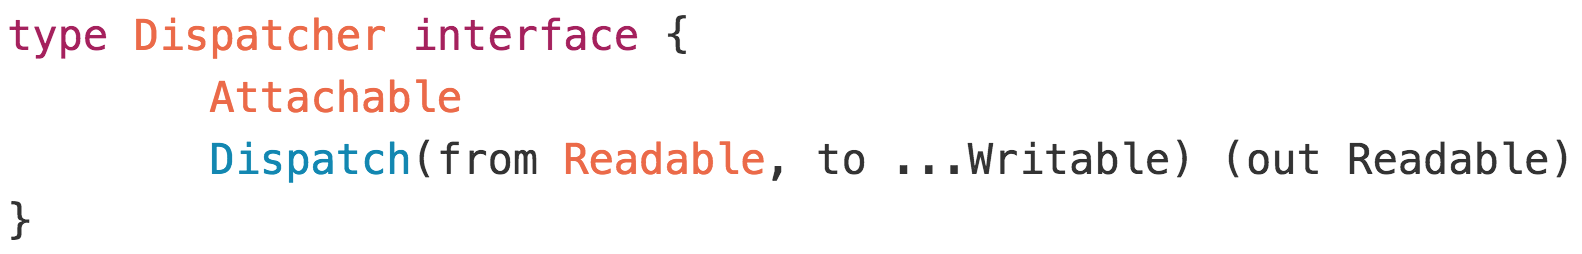
\includegraphics[width=0.85\textwidth]{dispatcher_interface}
  \centering
  \caption{Dispatcher Interface.}
  \label{code:rivers:dispatcher}
\end{figure}

Em particular dispatchers são úteis para classificar e agrupar dados em streams diferentes podendo processar cada stream utilizando lógicas específicas. Operações de partição são exemplos clássicos de Dispatchers em Rivers. A figura a seguir mostra um stream de números inteiros sendo particionado em dois outros streams, o primeiro contendo apenas números pares e o segundo números ímpares.

\begin{figure}[H]
  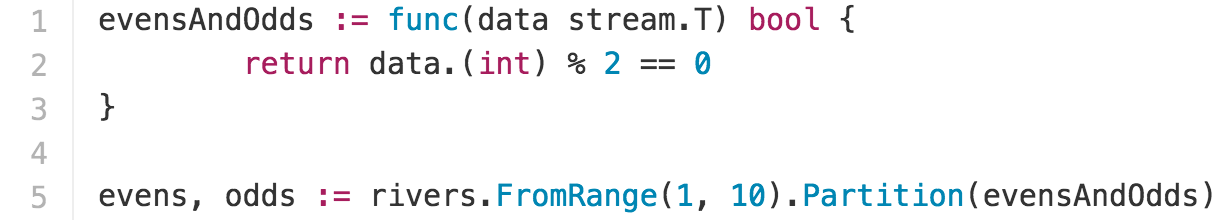
\includegraphics[width=0.85\textwidth]{partition_dispatcher}
  \centering
  \caption{Exemplo de particionamento de um stream de números inteiros.}
  \label{code:rivers:partition_dispatcher}
\end{figure}

Rivers API disponibiliza algumas implementações de dispatchers pré-definidas além da mencionanda anteriormente, como por exmplo Split que duplica um stream em dois outros idênticos útil para aplicar diferentes sequências de transformações concorrentes aos dados do stream como por exemplo salvar entidades na base de dados e concorrentemente indexar a informação em uma engine de busca ou salvar a informação em uma cache.

\subsection{O Contexto Global}
\label{sec:rivers:context}

Coordenar vários estágios concorrentes de um pipeline e garantir o término da execução mesmo na presença de erros são algumas das funções do contexto o qual é compartilhado por cada componente conectado ao pipeline. Um contexto implementa alguns mecanismos utilizados por cada componente descrito até o momento que permitem com que cada um deles possam sinalizar o término da execução devido a uma falha por exemplo, permitindo com que qualquer goroutine em execução possa suspender seu processamento verificando o canal Failure do contexto. Em casos em que um estágio do pipeline falhe causando uma situação de panic, o programa não finaliza inesperadamente uma vez que como descrito nos contratos de cada componente, a função de Recover do contexto é executada em modo defer como parte do processamento permitindo que o contexto capture o erro e sinalize a falha fechando o canal Failure causando com que cada componente suspenda sua execução liberando qualquer recurso de máquina utilizando até o momento, como conexões com base de dados, descritores de arquivos, etc.

\begin{figure}[H]
  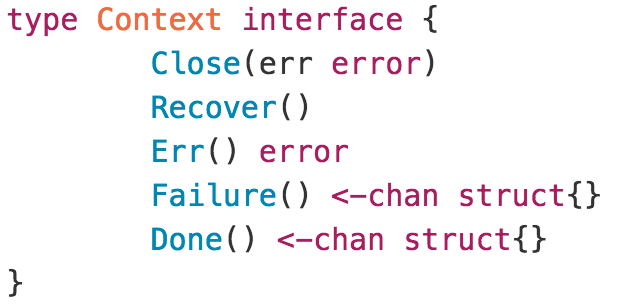
\includegraphics[width=0.45\textwidth]{context}
  \centering
  \caption{Context Interface.}
  \label{code:rivers:context}
\end{figure}

A figura acima representa a interface implementada por um contexto em Rivers. Qualquer componente conectado ao pipeline pode verificar o estado atual do pipeline através dos canais de comunicação Failure e Done do contexto ou requisitar o término da execução através do método Close de um contexto, provendo uma informação de erro opcional. Caso nenhum erro seja fornecido, a execução do pipeline é finalizada com sucesso mesmo que ainda haja elementos a serem produzidos. Este cenário é usual em operações de short-circuit como Find que sinaliza o término do pipeline assim que o primeiro elemento satisfazendo a condição de busca passe pelo estágio.

Em casos em que o canal Done do contexto é fechado qualquer Producer ou Transformer conectados ao pipeline de acordo com seus contratos devem encerrar seus processamentos liberando qualquer recurso alocado durante sua execução. Este mecanismo aonde cada componente é responsável por verificar o estado atual do contexto antes de realizar qualquer processamento e suspender a execução em caso de término devido a erros -- canal Failure -- ou devido ao término prematuro -- canal Done -- permite com que centenas de milhares de estágios concorrentes sejam conectados ao pipeline sem impactar na complexidade de gerência e coordenamento do pipeline, uma vez que sinalizar o término da execução de cada um destes estágios se resume no fechamento de um dos canais mencionados. Isso é possível devido ao excelente modelo de concorrência da linguagem Go que baseia-se na filosofia de compartilhamento de memória através da comunicação em vez de comunicar através do compartilhamento de memória.

\section{Suporte a Paralelização}
\label{sec:rivers:going_parallel}

Concorrência e paralelismo são conceitos similares porém diferentes, assim como abordado de maneira brilhante por Rob Pike em sua talk \cite{talk:rob_pike:concurrency_not_parallelism} Concurrency is not Parallelism. Estágios de um pipelines em Rivers são processados concorrentemente e cada estágio pode ainda ser paralelizado utilizando os recursos de hardware como multi-cores para atingir níveis extremos de paralelismo aumentado a eficiência do pipeline.

Rivers permite que certos tipos de Transformers possam ser paralelizados, como por exemplo um Map ou Each Transformer. Para atingir níveis aceitáveis de paralelismo Rivers replica o Transformer em questão em vários outros, tantos quanto for a capacidade do stream sendo consumido, por exemplo se um producer tem a capacidade de produção de 3 elementos o Transdormer seria replicado obtendo 3 instâncias paralelas. Cada novo Trnasformer consome dados do estágio anterior concorrentemente, produzindo seus resultados em um mesmo stream resultante que é consumido pelo estágio senguinte do pipeline. A figura \ref{fig:rivers:rivers_parallel} mostra como seria o fluxo de um pipeline com paralelismo ativado.

\begin{figure}[H]
  \includegraphics[width=0.55\textwidth]{rivers_parallel}
  \centering
  \caption{Fluxo de um Pipeline com Paralelismo ativado.}
  \label{fig:rivers:rivers_parallel}
\end{figure}

Essa solução permite aliviar bottlenecks relacionados a estes tipos de Transformers. O código \ref{code:rivers:parallel_pipeline} mostra um exemplo de pipeline sendo executado sequencialmente e outro com paralelismo ativado:

\begin{figure}[H]
  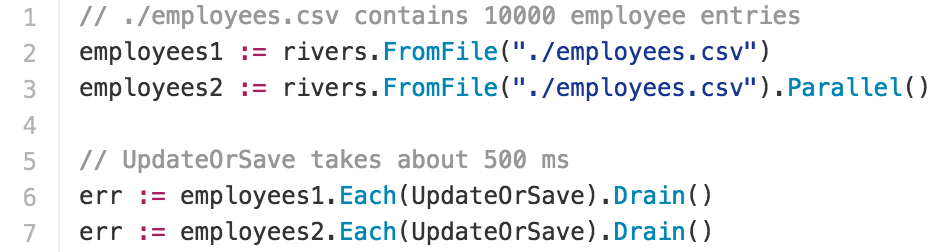
\includegraphics[width=0.8\textwidth]{parallel_pipeline}
  \centering
  \caption{Exemplo de Paralelismo em Rivers.}
  \label{code:rivers:parallel_pipeline}
\end{figure}

No exemplo acima, dois pipelines são criados para processar um arquivo CSV contendo 10000 entradas com informações de empregados de uma determinada empresa. Para cada empregado deve-se verificar sua existência na base de dados atualizar determinada informação caso exista, ou criar uma nova entrada para o empregado correspondente. Esse procedimento leva em torno de 500 ms por empregado. O primeiro pipeline por não utilizar paralelismo levaria um tempo total de aproximadamente 1.38 horas para finalizar o processamento. Já o segundo pipeline, por ativar o uso de paralelismo, Rivers replica o estágio Each para cada entrada de Employee extraída do arquivo CSV executando cada estágio concorrentemente distribuindo a carga de trabalho em diferentes threads fazendo o uso de todos os cores disponíveis na máquina. O tempo total de execução do segundo pipeline medido em uma máguina com 8 cores foi de aproximadamente 2.58 segundos.